\subsection{Το σύστημα \lat{Lorenz}}
Tο συστημα \lat{Lorenz}, που μελετήθηκε για πρώτη φορά από τον \lat{Edward Lorenz} στο έργο του \textit{\lat{Deterministic nonperiodic flow}}, \lat{\cite{LOR}}, είναι ένα σύστημα που αποτελείται από συνήθεις διαφορικές εξισώσεις και αποτελεί ένα αξιοσημείωτο παράδειγμα χαοτικού προβλήματος.

Για συγκεκρίμενες τιμές των παραμέτρων, το σύστημα συμπεριφέρεται χαοτικά. Μικρές μεταβολές στις αρχικές συνθήκες καταλήγουν σε τελείως διαφορετική λύση του προβλήματος, που παραμένει ωστόσο ντετερμινιστικό.

Ο ελκυστήρας του \lat{Lorenz}, όπως είναι γνωστό το σύστημα, αποτελεί μία απλοποιημένη μορφή ενός συστήματος εξισώσεων που περιγράφουν την διδιάστατη ροή ενός ρευστού, με ομοίομορφο πάχος $H$ και διαφορά θερμοκρασίας $ΔΤ$, υπό την επήρεια της βαρυτικής επιτάχυνσης $g$, με άνωση $α$, συντελεστή θερμικής μετάδοσης $κ$ και κινηματικό ιξώδες $ν$, \lat{\cite{TABOR}}
\begin{align}
    \dfrac{\partial}{\partial{t}}\left(\nabla^{2} φ\right) &= \dfrac{\partial ψ}{\partial z} \dfrac{\partial}{\partial x}\left(\nabla^{2} ψ\right) - \dfrac{\partial ψ}{\partial x} \dfrac{\partial}{\partial z}\left(\nabla^{2} ψ\right) + ν\nabla^{2}\left(\nabla^{2}ψ\right) + gα\dfrac{dT}{dx} \\
    \dfrac{\partial T}{\partial t} &= \dfrac{\partial{T}}{\partial{z}}\dfrac{\partial{ψ}}{\partial{x}} - \dfrac{\partial{θ}}{\partial{x}}\dfrac{\partial{ψ}}{\partial{z}} + κ\nabla^{2}T + \dfrac{ΔT}{H}\dfrac{\partial{ψ}}{\partial{x}}
\end{align}

όπου $ψ$ η ροϊκή συνάρτηση τέτοια ώστε το διάνυσμα της ταχύτητα $\textbf{u}=\left(u, w\right)$ είναι
\begin{align}
    u &= \dfrac{\partial{ψ}}{\partial{z}} \\
    w &= -\dfrac{\partial{ψ}}{\partial{x}}
\end{align}

Ο \lat{Lorenz} ανακάλυψε τυχαία ότι σε ένα απλοποιημένο σύστημα, του οποίου η λύση είναι συγκεκριμένης μορφής, παρουσιαζεται χαοτική συμπεριφορά
\begin{equation}
    \begin{cases}
        \dfrac{dx}{dt} &= σ\left(y - x\right) \\
        \dfrac{dy}{dt} &= x\left(ρ - z\right) - y \\
        \dfrac{dz}{dt} &= xy - βz 
    \end{cases}
\end{equation}

Το απλοποιημένου του σύστημα συσχετίζει τις ιδιότητες ενός διδιάστατου ρευστου στρώματος, όπου το $x$ είναι ανάλογο του ρυθμού μετάδοσης, το $y$ είναι ανάλογο της διαφοράς θερμοκρασίας κατά μήκος και το $z$ είναι ανάλογο της κατακόρυφης κατανομής της θερμοκρασίας.

Ακόμα εισήγαγε τις θετικές παραμέτρους $σ$, $ρ$ που είναι ανάλογες του αριθμού \lat{Prandtl} και του αριθμού \lat{Rayleigh}, καθώς και το $β$ που είναι χαρακτηριστικό για των φυσικών διαστάσεων του ρευστού στρώματος.

Στο σύστημα εμφανίζονται τρία κρίσιμα σημεία. Το πρώτο $\left(0, 0, 0\right)$ που αντιστοιχεί σε μηδενική μετάδοση και τα 
\begin{align}
    \left( \sqrt{β\left(ρ-1\right)} , \sqrt{β\left(ρ-1\right)} , ρ-1\right) \\
    \left( -\sqrt{β\left(ρ-1\right)} , -\sqrt{β\left(ρ-1\right)} , ρ-1\right)
\end{align}
που αντιστοιχούν σε σταθερή μετάδοση θερμότητας. Το ζεύγος των σημείων είναι ευσταθές μόνο αν 
\begin{equation}
    ρ < σ\dfrac{σ+β+3}{σ-β-1} \Rightarrow σ>β+1
\end{equation}

Οι τιμές που ο \lat{Lorenz} επέλεξε για τις παραμέτρους, για τις οποίες παρουσιάζεται χαοτική συμπεριφορά, είναι
\begin{align}
    σ &= 10 \\
    β &= 8/3 \\
    ρ &= 23
\end{align}

Το σύστημα είναι δύσκολο να αναλυθεί και συνήθως είναι πιο εύκολη η οπτικοποιήση του, μέσω της λύσης του με κάποια υπολογιστική τεχνική. Το οπτικό αποτέλεσμα εμφανίζει τη μορφή μια πεταλούδας ή του αριθμού 8 και αυτός είναι ο λόγος που πήρε το όνομά του το \textit{φαίνομενο της πεταλούδας}, όρο τον οποίο χρησιμοποίησε για πρώτη φορά ο \lat{Edward Lorenz}.

\subsection{Υπολογιστική Επίλυση}

Το σύστημα των διαφορικών εξισώσεων μπορεί να λυθεί εύκολα κάνοντας χρήση μίας υπολογιστικής μεθόδου. Για την παρούσα εργασία επιλέχθηκε η επίλυση μέσω της μεθόδου \textit{\lat{LSODA}}, κυρίως λόγω της της ευκολίας στην υλοποίηση, αλλά και της δυνατότητας του αλγορίθμου να προσαρμόζεται στο σύστημα και να προσαρμόζει και το βήμα ολοκλήρωσης (\lat{\textit{variable step size intergration}}).

Για την υπολογιστική επίλυση χρησιμοποιήθηκε η γλώσσα \textit{\lat{Python}} και το πακέτο αριθμητικής ολοκλήρωσης διαφορικών εξισώσεων \textit{\lat{scipy.intergrate.odeint}}, που χρησιμοποιεί τη βιβλιοθήκη της \textit{\lat{LSODA}} που προέρχεται από τη \textit{\lat{FORTRAN}}. Στο \lat{documentation} της βιβλιοθήκης αριθμητικής ολοκλήρωσης διαφορικών εξισώσεων \textit{\lat{scipy.intergrate.odeint}} περιγράφεται ότι
\begin{displayquote}
    \selectlanguage{english}
    \textit{Solve a system of ordinary differential equations using lsoda from the FORTRAN library odepack.}  \\
    \textit{Solves the initial value problem for stiff or non-stiff systems of first order ode-s:}
    \begin{verbatim}
        dy/dt = func(y, t, ...)  [or func(t, y, ...)]
    \end{verbatim}
    \textit{where y can be a vector.}
\end{displayquote}

Αντίστοιχα το \lat{documentation} της \lat{LSODA} αναφέρει ότι
\begin{displayquote}
    \selectlanguage{english}
    \textit{\textbf{LSODA}, written jointly with L. R. Petzold, solves systems dy/dt = f with a dense or banded Jacobian when the problem is stiff, but it automatically selects between nonstiff (Adams) and stiff (BDF) methods. It uses the nonstiff method initially, and dynamically monitors data in order to decide which method to use.}
\end{displayquote}

\subsection{Αλγόριθμος επίλυσης}
\selectlanguage{english}
\lstset{style=nonums}
\lstinputlisting[nolol=true, language=Python, caption=Lorenz System Solver]{lorenz.py}

\subsection{Γραφικό Περιβάλλον}
Για τη δημιουργία ενός απλού λογισμικού με γραφική διεπαφή χρήστη (\lat{GUI}) έγινε χρήση της γλώσσας προγραμματισμού \lat{Python}. Μέσω της γραφικής διεπαφής ο χρήστης έχει τη δυνατότητα να εισάγει διάφορα αρχικά σημεία και να λάβει μία κινούμενη τριδιάστατη επίλυση του συστήματος \lat{Lorenz}.
\subsubsection{Κυρίως παράθυρο}
Στο σχήμα \ref{fig:lorenz-gui} φαίνεται το κυρίως παράθυρο του λογισμικού. Το παράθυρο αποτελείται από δύο βασικά μέρη. Το πρώτο, στα αριστερά, περιλαμβάνει όλες τις βασικές λειτουργίες, καθώς και τις παραμετροποιήσεις που μπορεί να εισάγει στο σύστημα ο χρήστης. Στο δεύτερο μισό, στα δεξιά, εμφανίζεται η γραφική επίλυση του συστήματος, της οποία την απεικόνιση μπορεί να επεξεργαστεί ο χρήστης.
\begin{figure}[!h]
    \centering
    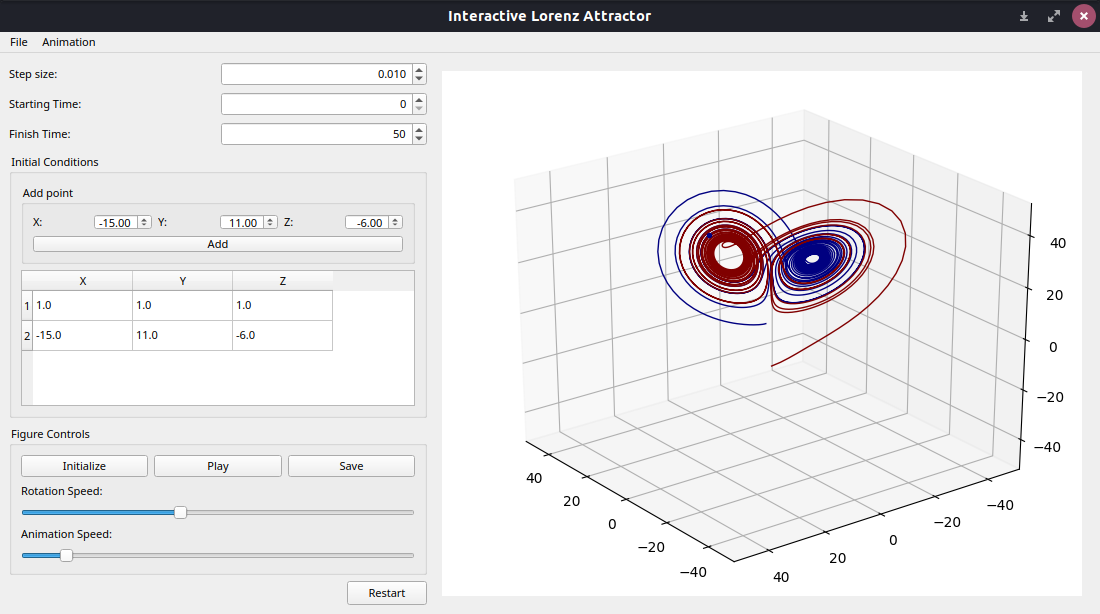
\includegraphics[scale=0.4]{lorenz-gui}
    \caption{Γραφική διεπαφή χρήστη του λογισμικού \lat{"Interactive Lorenz Attractor"}.}
    \label{fig:lorenz-gui}
\end{figure}

Ο χρήστης επιλέγοντας πρώτα τις συντεταγμένες του αρχικού σημείου, το εισάγει στη λίστα με το κουμπί \textbf{\lat{Add}}. Με διπλό κλικ σε οποιοδήποτε αντικείμενο της λίστας, μπορεί να διαγράψει ένα αρχικό σημείο. Με τα κουμπια \textbf{\lat{Initialize}} και \textbf{\lat{Play/Stop}}, καθώς και με τους κυλιόμενους δείκτες, είναι δυνατή η παραμετροποιήση της εμφάνισης του διαγράμματος. Τέλος, προσφέρεται η δυνατότητα αποθήκευσης, ως αρχείο εικόνας, του διαγράμματος, οποιαδήποτε στιγμη, όπως φαίνεται στο σχήμα. 
\begin{figure}
    \centering
    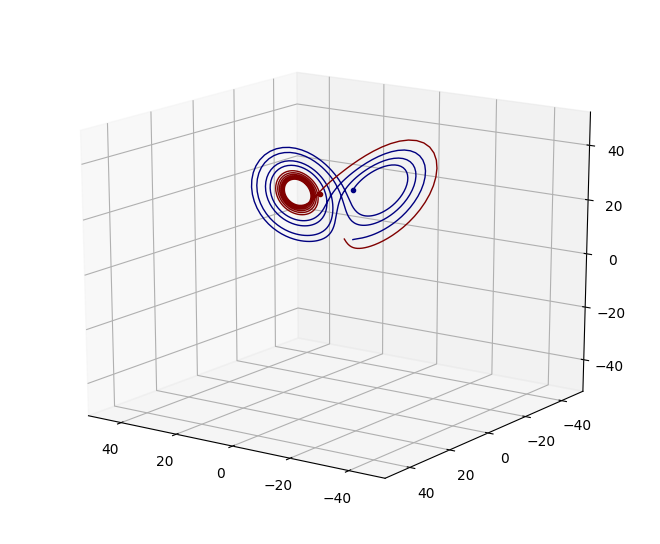
\includegraphics[scale=0.7]{lorenz-out}
    \caption{Επίλυση συστήματος με αρχικά σημεία $(-5,0,10)$ και $(5,-10,6)$.}
    \label{fig:lorenz-out}
\end{figure}